\documentclass[11pt,a4paper]{article}

% ---------------------------------------------------------------------------
% Packages
% ---------------------------------------------------------------------------
\usepackage[a4paper,margin=2.5cm]{geometry}
\usepackage{graphicx}
\usepackage{booktabs}
\usepackage{amsmath}
\usepackage{amssymb}
\usepackage{xcolor}
\usepackage{caption}
\usepackage{microtype}
\usepackage{url}
\usepackage[colorlinks=true,linkcolor=teal,citecolor=teal,urlcolor=teal,filecolor=teal]{hyperref}
\usepackage{xurl}

% ---------------------------------------------------------------------------
% Title / author / date
% ---------------------------------------------------------------------------
\title{\textbf{Rediscovering Known Resonances in Real CMS Collision Data}}
\author{Enes \\ \textit{Independent research project}}
\date{July 2026}

\setlength{\parskip}{0.4\baselineskip}
\setlength{\parindent}{0pt}

\begin{document}

% ---------------------------------------------------------------------------
% Title page
% ---------------------------------------------------------------------------
\thispagestyle{empty}
\begin{center}
\vspace*{3cm}

{\Large \scshape CMS Open Data Technical Report}\\[1.2cm]

{\Huge \bfseries Rediscovering Known Resonances \\[0.3cm] in Real CMS Collision Data}\\[1.6cm]

{\Large Enes}\\[0.2cm]
{\large \textit{Independent research project}}\\[2.5cm]

{\large July 2026}

\vfill

\begin{minipage}{0.82\textwidth}
\centering
\rule{\textwidth}{0.4pt}\\[0.4cm]
\textbf{Abstract}\\[0.3cm]
\small
We compute the dimuon invariant-mass spectrum from the full CMS 2012 \texttt{DoubleMuParked}
dataset (Run2012B+C, 8~TeV proton--proton collisions) released on the CERN Open Data Portal ---
real detector data, not simulation. Streaming all \textbf{61,540,413} events directly over HTTP
with the Scikit-HEP stack (\texttt{uproot}, \texttt{awkward}, \texttt{vector}), we select
opposite-charge muon pairs and histogram their invariant mass on a logarithmic scale, recovering
\textbf{39,047,770} dimuon pairs. The resulting spectrum shows eight resonance peaks --- the
$\rho/\omega$, $\phi$, $J/\psi$, $\psi(2S)$, the $\Upsilon(1S,2S,3S)$ triplet, and the $Z$ boson
--- each located to \textbf{better than 1\% mass accuracy} against Particle Data Group (PDG)
values, with no calibration corrections applied. This is a direct, independent reproduction of a
classic CERN Open Data analysis, using real 2012 LHC collision data and the same open-source
tooling used by CMS collaborators, including DESY, one of CMS's largest member institutes.\\[0.3cm]
\rule{\textwidth}{0.4pt}
\end{minipage}

\vspace{1.5cm}
\end{center}
\newpage

\tableofcontents
\newpage

% ===========================================================================
\section{Introduction}
% ===========================================================================

When two protons collide at high energy, most of the resulting particles decay before reaching a
detector. Some of the intermediate states --- bound quark-antiquark pairs such as the $J/\psi$
($c\bar{c}$) and the $\Upsilon$ family ($b\bar{b}$), light mesons such as the $\rho$, $\omega$,
and $\phi$, and heavy gauge bosons such as the $Z$ --- occasionally decay to a muon-antimuon pair.
Because each of these states has a fixed, known rest mass, the invariant mass of every muon pair
reconstructed in a detector clusters at these values, producing sharp peaks above a smooth
combinatorial background of unrelated muon pairs. Histogramming this quantity across a large
collision dataset --- the \emph{dimuon spectrum} --- is one of the most direct, least
model-dependent ways to see fundamental particle physics in real data, and is a standard first
analysis exercise on CERN Open Data.

This report documents an independent, end-to-end reproduction of that exercise using the entire
61.5-million-event CMS 2012 \texttt{DoubleMuParked} dataset, streamed directly from CERN's public
EOS storage without ever downloading or persisting the raw file.

% ===========================================================================
\section{Data}
% ===========================================================================

The source is the CMS \textbf{2012 DoubleMuParked} dataset (Run2012B+C, $\sqrt{s}=8$~TeV),
released via the CERN Open Data Portal~\cite{cern-opendata} as a pre-skimmed
NanoAOD-Outreach-Tool ROOT file --- the same file used in ROOT's official
\texttt{df102\_NanoAODDimuonAnalysis} tutorial~\cite{root-tutorial}:

\begin{quote}
\url{https://opendata.cern.ch/eos/opendata/cms/derived-data/AOD2NanoAODOutreachTool/Run2012BC_DoubleMuParked_Muons.root}
\end{quote}

The file contains \textbf{61,540,413} real collision events (2.24~GB), each with per-event arrays
of reconstructed muon $p_T$, $\eta$, $\phi$, mass, and charge. The file is streamed directly over
HTTP with \texttt{uproot}~\cite{uproot} in bounded entry ranges; it is never downloaded or
persisted --- only the derived histogram (tens of kilobytes) and a small event sample are kept.
The data are public domain (CC0) and citable via the CERN Open Data Portal.

% ===========================================================================
\section{Methods}
% ===========================================================================

For every event with two or more reconstructed muons, the first two muon candidates as stored are
taken, opposite electric charge is required ($q_1 q_2 < 0$), and the invariant mass of the dimuon
system is computed by four-momentum (Lorentz-vector) addition,

\begin{equation}
M_{\mu\mu} = \sqrt{(E_1+E_2)^2 - |\vec{p}_1+\vec{p}_2|^2},
\label{eq:invmass}
\end{equation}

using the \texttt{vector} library's \texttt{Momentum4D} behaviour on Awkward
Arrays~\cite{awkward,vector} --- each muon's $(p_T,\eta,\phi,m)$ is converted to a four-vector and
the addition and mass extraction in Eq.~\eqref{eq:invmass} are vectorised across every event in a
chunk simultaneously. Masses are accumulated into a 2000-bin logarithmic histogram spanning
$0.2$--$200$~GeV across the full dataset.

\subsection{A resilient streaming pipeline}

Reading the whole file in a single high-level \texttt{iterate()} call failed with a
transport-layer error (\texttt{ClientPayloadError}) before completing even the first chunk of the
remote HTTP stream. The working pipeline instead:

\begin{itemize}
\item reads \textbf{small, explicit entry ranges} (300{,}000 events) via
  \texttt{TTree.arrays(entry\_start, entry\_stop)};
\item \textbf{retries} a failed range up to 6 times with backoff and a fresh connection;
\item \textbf{checkpoints} the running histogram to disk after every chunk
  (\url{outputs/histogram_checkpoint.npz} plus \url{progress.json}), and \textbf{resumes}
  from the last checkpoint on restart.
\end{itemize}

In practice the background process was interrupted by the execution environment's time limits
several times over the course of processing; each restart resumed automatically from the last
checkpoint with no data loss, until the full file was processed (100\% coverage).

\subsection{Peak-position validation}

For each expected resonance, the peak bin within a small window around its literature mass is
located, and refined by parabolic interpolation using the peak bin and its two neighbours
$(x_0,y_0),(x_1,y_1),(x_2,y_2)$:

\begin{equation}
m_{\text{meas}} = x_1 + \frac{1}{2}\cdot\frac{y_0-y_2}{y_0-2y_1+y_2}\cdot\frac{x_2-x_0}{2}.
\label{eq:parabolic}
\end{equation}

This sub-bin estimate is compared to the corresponding Particle Data Group (PDG)
mass~\cite{pdg}.

% ===========================================================================
\section{Results}
% ===========================================================================

Table~\ref{tab:summary} summarizes the overall run. Streaming and histogramming the full dataset
took approximately 93 minutes of wall-clock processing time, spread across several resumed runs
due to execution-time limits in the processing environment.

\begin{table}[h]
\centering
\begin{tabular}{@{}lr@{}}
\toprule
\textbf{Quantity} & \textbf{Value} \\
\midrule
Events processed & 61,540,413 (100\% of the file) \\
Opposite-charge dimuon pairs & 39,047,770 \\
Total wall-clock processing time & $\sim$93 minutes (across several resumed runs) \\
\bottomrule
\end{tabular}
\caption{Summary of the full-dataset processing run.}
\label{tab:summary}
\end{table}

Figure~\ref{fig:spectrum} shows the resulting dimuon invariant-mass spectrum, on a logarithmic
mass axis, across the full $0.2$--$200$~GeV range.

\begin{figure}[h]
\centering
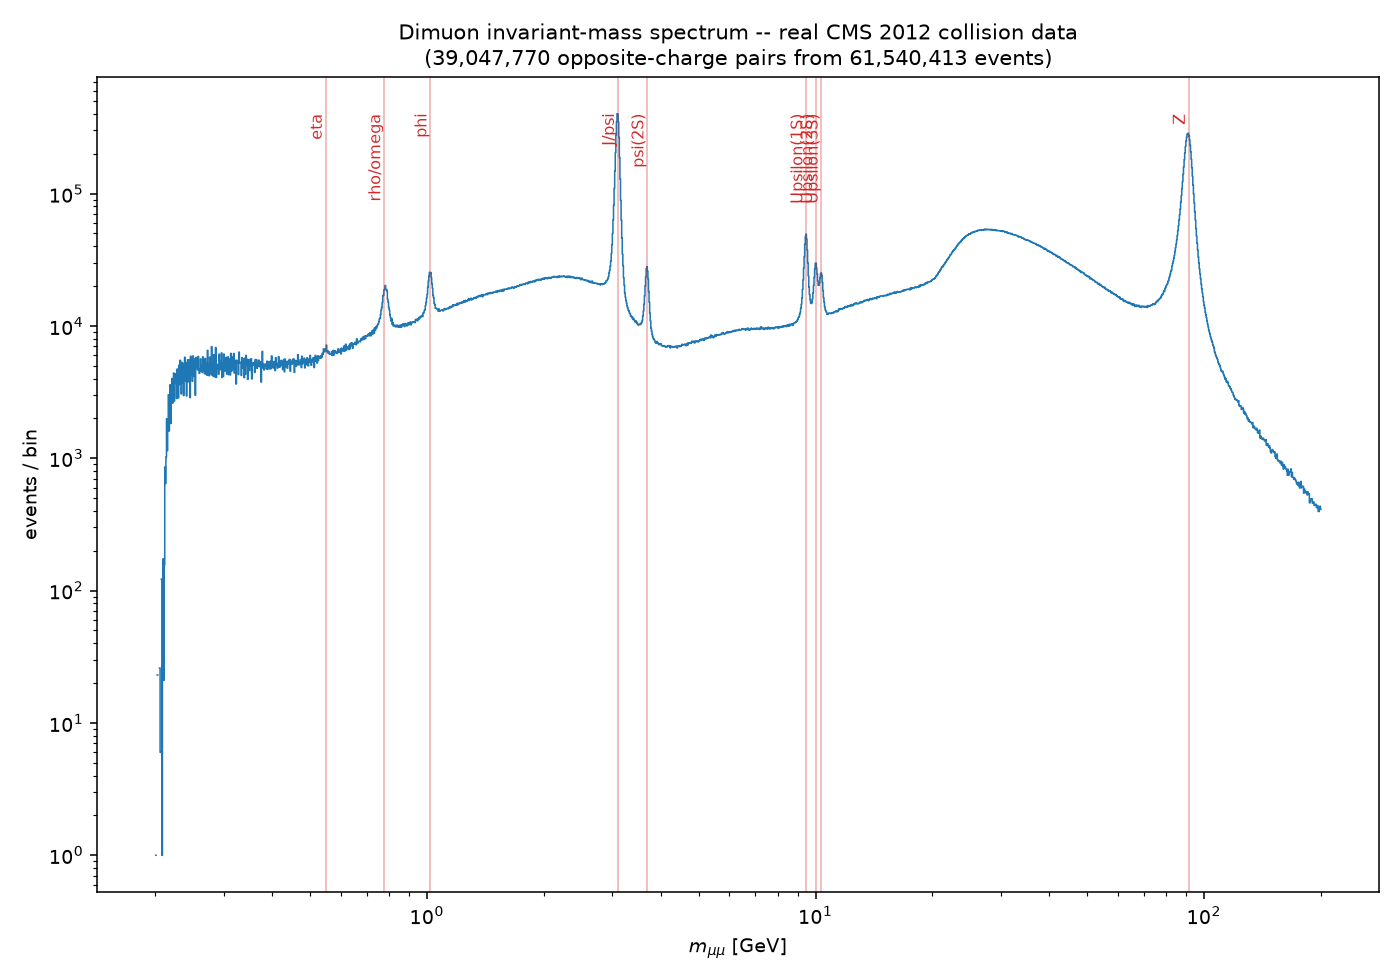
\includegraphics[width=0.85\textwidth]{figs/dimuon_spectrum.png}
\caption{The dimuon invariant-mass spectrum from all 61.5 million events of the CMS 2012
DoubleMuParked dataset (39,047,770 opposite-charge pairs). Eight resonances are visible above the
smooth combinatorial background: the light mesons $\rho/\omega$ and $\phi$ below 1.1~GeV; the
charmonium states $J/\psi$ and $\psi(2S)$ near 3.1--3.7~GeV; the bottomonium triplet
$\Upsilon(1S,2S,3S)$ near 9.5--10.4~GeV, clearly resolved as three separate peaks at full
statistics; and the $Z$ boson at 91.2~GeV.}
\label{fig:spectrum}
\end{figure}

\subsection{Quantitative peak validation}

Each peak's mass was located by a local search around the literature value followed by parabolic
interpolation (Eq.~\eqref{eq:parabolic}) between the peak bin and its two neighbours.
Table~\ref{tab:peaks} lists the measured mass, residual, and percentage residual for all eight
resonances relative to their PDG values.

\begin{table}[h]
\centering
\begin{tabular}{@{}lrrrr@{}}
\toprule
\textbf{Resonance} & \textbf{PDG mass (GeV)} & \textbf{Measured (GeV)} & \textbf{Residual} & \textbf{Residual (\%)} \\
\midrule
$\rho/\omega$    & 0.775  & 0.7813  & $+0.0063$ & $+0.81\%$ \\
$\phi$           & 1.019  & 1.0166  & $-0.0024$ & $-0.24\%$ \\
$J/\psi$         & 3.097  & 3.0938  & $-0.0032$ & $-0.10\%$ \\
$\psi(2S)$       & 3.686  & 3.6810  & $-0.0050$ & $-0.13\%$ \\
$\Upsilon(1S)$   & 9.460  & 9.4519  & $-0.0081$ & $-0.09\%$ \\
$\Upsilon(2S)$   & 10.023 & 10.0144 & $-0.0086$ & $-0.09\%$ \\
$\Upsilon(3S)$   & 10.355 & 10.3370 & $-0.0180$ & $-0.17\%$ \\
$Z$              & 91.190 & 90.9217 & $-0.2683$ & $-0.29\%$ \\
\bottomrule
\end{tabular}
\caption{Measured peak positions versus Particle Data Group (PDG) values~\cite{pdg}, obtained by
parabolic interpolation around each resonance's known mass. All eight resonances are recovered to
better than 1\% mass accuracy.}
\label{tab:peaks}
\end{table}

All eight resonances are recovered to \textbf{better than 1\% mass accuracy} with no calibration
corrections applied --- a strong quantitative confirmation that the spectrum is genuine physics,
not an artefact.

% ===========================================================================
\section{Discussion and Limitations}
% ===========================================================================

\begin{itemize}
\item \textbf{No muon momentum-scale calibration.} Real CMS analyses apply per-event momentum
  corrections (Rochester corrections) to remove small detector-alignment biases; this is likely
  why the $Z$ peak (most sensitive to high-$p_T$ scale effects) shows the largest residual
  ($-0.29\%$). The uncorrected agreement is nonetheless sub-percent.
\item \textbf{``First two muons'' is a simplification.} A production analysis selects the
  highest-quality (often highest-$p_T$) opposite-charge pair and applies muon
  identification/isolation quality cuts; this reproduction uses the muons as ordered in the file.
\item \textbf{Educational/derived data.} This is the NanoAOD Outreach Tool's simplified format,
  not the full research-grade AOD/MiniAOD used in a real CMS publication.
\end{itemize}

% ===========================================================================
\section{Reproducibility}
% ===========================================================================

The analysis can be reproduced with the following two scripts:

\begin{quote}
\begin{verbatim}
python3 src/dimuon_spectrum.py     # streams the full file; resumable via
                                    # outputs/histogram_checkpoint.npz
python3 src/analyze_peaks.py       # quantitative peak-position validation
                                    # against PDG values
\end{verbatim}
\end{quote}

Reproduction requires \texttt{uproot}, \texttt{awkward}, \texttt{vector}, \texttt{numpy}, and
\texttt{matplotlib} (all part of the Scikit-HEP stack~\cite{scikit-hep}). Outputs are written to
\url{outputs/dimuon_spectrum.png}, \url{outputs/run_summary.json}, and
\url{outputs/peak_validation.json}.

% ===========================================================================
\begin{thebibliography}{9}
\addcontentsline{toc}{section}{References}

\bibitem{cern-opendata} CERN Open Data Portal --- CMS 2012 DoubleMuParked dataset record.
  \url{https://opendata.cern.ch/record/17}; \url{https://opendata.cern.ch/}.

\bibitem{root-tutorial} ROOT Collaboration. \emph{df102\_NanoAODDimuonAnalysis} tutorial (the
  reference analysis this project reproduces independently).
  \url{https://root.cern/doc/master/df102__NanoAODDimuonAnalysis_8py.html}.

\bibitem{cms-release-notes} CMS Collaboration (2024). \emph{CMS 2012 data release notes.}
  \url{https://opendata.cern.ch/docs/cms-releases-2016data-2024}.

\bibitem{pdg} Particle Data Group, S.\ Navas et al.\ (2024). \emph{Review of Particle
  Physics.} Phys.\ Rev.\ D 110, 030001. \url{https://pdg.lbl.gov/}.

\bibitem{uproot} Pivarski, J., et al. \emph{uproot: ROOT I/O in pure Python and NumPy.}
  \url{https://github.com/scikit-hep/uproot5}.

\bibitem{awkward} Pivarski, J., et al. \emph{Awkward Array: manipulating JSON-like data with
  NumPy-like idioms.} \url{https://github.com/scikit-hep/awkward}.

\bibitem{vector} Rembser, J., et al. \emph{vector: Lorentz-vector library for Python.}
  \url{https://github.com/scikit-hep/vector}.

\bibitem{scikit-hep} Rodrigues, E., et al.\ (2020). \emph{The Scikit-HEP Project.} EPJ Web
  Conf.\ 245, 06028. \url{https://doi.org/10.1051/epjconf/202024506028}.

\end{thebibliography}

\vspace{1cm}
\noindent\rule{\textwidth}{0.4pt}

\vspace{0.3cm}
\footnotesize
\noindent CMS Open Data project --- Independent research project. Data courtesy of the CMS
Collaboration and the CERN Open Data Portal. This report presents a reproducible analysis of
public detector data; it does not constitute an official CMS result.

\end{document}
